\documentclass[11pt]{article}

\usepackage[margin=0.82in]{geometry}
\usepackage{amsmath,amssymb,bm}
\usepackage{booktabs}
\usepackage{graphicx}
\usepackage{hyperref}
\usepackage{xcolor}
\usepackage[T1]{fontenc}

\hypersetup{
  colorlinks=true,
  linkcolor=blue!55!black,
  citecolor=blue!55!black,
  urlcolor=blue!55!black
}
\newcommand{\code}[1]{\texttt{#1}}
\newcommand{\RefGH}{Ref--GH}
\newcommand{\M}{\mathcal{M}}
\newcommand{\CI}{\mathcal{C}_{IAB}}
\newcommand{\CIJ}{\mathcal{C}_{IJAB}}
\newcommand{\CGH}{\mathcal{C}_{A}}
\newcommand{\notrun}{\textcolor{red!65!black}{not run}}
\newcommand{\passed}{\textcolor{green!45!black}{passed}}
\newcommand{\failed}{\textcolor{red!65!black}{failed}}

\title{Fixed-Stitch Ref--GH Failure Evidence and a Controlled\\
Gaussian-Reference / Full-$\gamma_2$ Investigation}
\author{AthenaK vacuum Ref--GH campaign report}
\date{24 August 2026}

\begin{document}
\maketitle

\begin{abstract}
This report packages the compact evidence from the paused Aurora fixed-core
Schwarzschild continuation campaign and turns its formulation audit into a
controlled next-step design.  The feedback run T4 failed closed at
$t=3.70126M$; the independent prescribed run T5 became ill-conditioned at RK
stage time $t=3.18677M$.  Growth is localized near $r=0.45$--$0.56M$, within
the artificial $0.30$--$0.60M$ wormhole/trumpet stitch, while measured
characteristic travel excludes the $24M$ outer boundary.  Feedback delays
failure in coordinate time but is worse than the prescribed path at equal
activation near the transition.  The present code has $\gamma_0>0$ but
$\gamma_2=0$; its ``standard'' $\Phi$ ordering is not the complete
$\gamma_2$-damped first-order generalized-harmonic system.

The proposed follow-up separates two hypotheses: replace the narrow compact
stitch with a broad Gaussian-localized Schwarzschild reference, then add the
complete standard $\gamma_2$ constraint additions in the moving reference
frame.  No Gaussian or nonzero-$\gamma_2$ evolution has yet been run.  This
document therefore establishes neither trumpet stability nor convergence; it
defines the derivation, oracles, fixed matrices, and fail-closed gates required
to test those claims.
\end{abstract}

\section{Status and claim boundary}

The report branch was created only after fetching the remote parent and
confirming exact equality:
\begin{center}
\begin{tabular}{ll}
\toprule
parent branch & \code{codex/ref-gh-feedback-continuation-20260823} \\
parent/local/upstream/remote SHA & \code{e5579269f2e979d246ab162a288b140e7076d666} \\
report branch & \code{codex/ref-gh-gaussian-reference-gamma2-20260824} \\
T5 source SHA & \code{0189d495058e09a53ca36a31f08ab924bc496582} \\
T5 executable SHA-256 & \code{7496ae64fe8a57c4f3111884bd04be94}\ldots \\
\bottomrule
\end{tabular}
\end{center}
The complete executable hash and run provenance are retained in the compact
artifact tree.  The final pushed branch SHA is deliberately reported by Git
rather than embedded self-referentially in this PDF.  A live
\code{qstat -u hzhu} check during packaging returned no entries, confirming
that no Aurora campaign job remained queued or running.

\paragraph{Established.}
The T0--T2 source/algebra/moving-reference gates, a twelve-PVC execution gate,
rank-to-tile mapping, and checkpoint/restart continuity passed for their named
workloads.  T4 and T5 both failed on the same $328$-MeshBlock,
$[-24M,24M]^3$ medium SMR mesh.  Their failure maxima are deep inside the
finest region and causally disconnected from the outer faces.

\paragraph{Not established.}
No result supports stable full activation, a stationary trumpet hold,
resolution convergence, long-time stability, production performance, or a
causal attribution to one formulation term.  No Gaussian reference,
GH-compatible mismatched-reference initializer, or $\gamma_2$ implementation
exists on this report branch.  All proposed matrices in Sec.~\ref{sec:gates}
therefore remain \notrun.

\section{Controlling fixed-stitch evidence}

\subsection{Runs and outcomes}

Both discriminators used eight Aurora nodes, 96 distinct PVC tiles, one rank
per tile, and the identical physical grid.  The minimum spacing was
$\Delta x_{\min}=M/24$.  No floor, clipping, stuffing, reset, or threshold
relaxation concealed either failure.

\begin{table}[h]
\centering
\caption{Definitive medium-grid outcomes.  History output precedes the fatal
RK-stage check.}
\begin{tabular}{lrrrrl}
\toprule
run & last history $t/M$ & fatal stage $t/M$ & last $\xi$ & $S(\xi)$ & outcome \\
\midrule
T4 feedback & 3.652312 & 3.70126 & 0.683571 & 0.814516 & constraint-growth veto \\
T5 prescribed & 3.150078 & 3.18677 & 0.787520 & 0.932046 & invalid relative metric \\
\bottomrule
\end{tabular}
\end{table}

Figure~\ref{fig:time} shows the complete committed histories.  T5 traverses
the reference path faster and reaches substantially larger conditioning,
relative boost, and native constraints by its final output.  This is a
time-domain observation, not evidence that feedback repairs the formulation.

\begin{figure}[p]
\centering
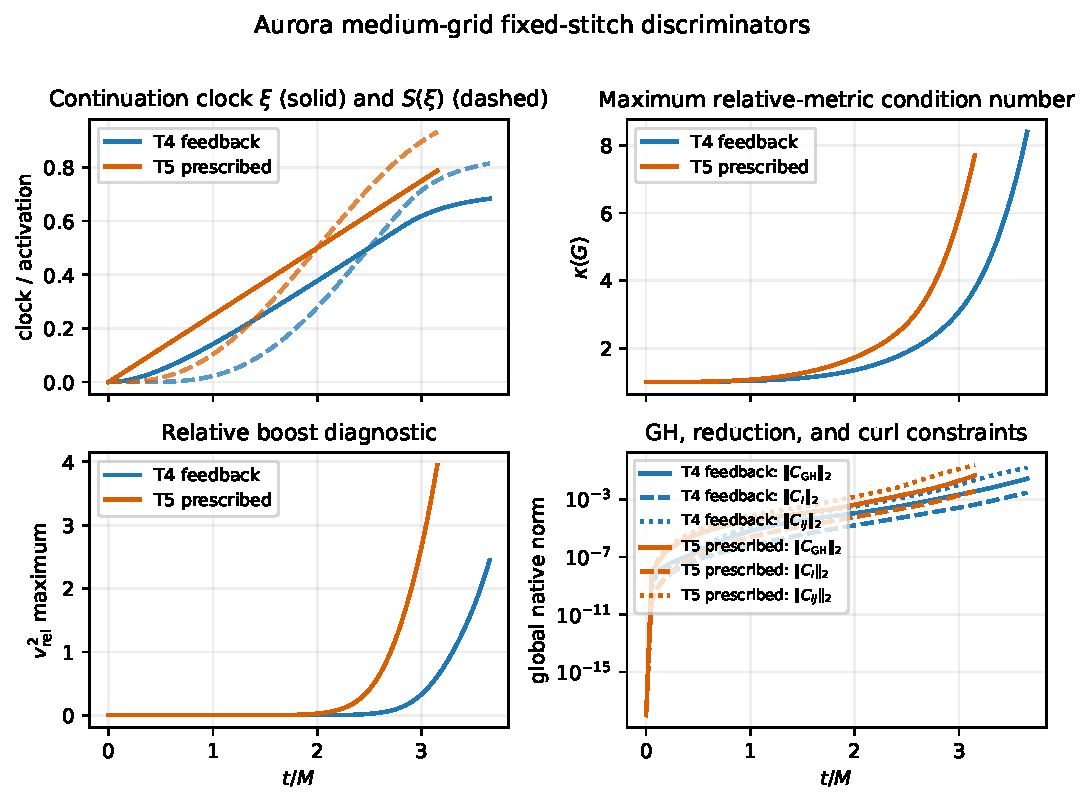
\includegraphics[width=0.96\textwidth]{fo_gh_artifacts/ref_gh_gaussian_reference_gamma2_20260824/figures/t4_t5_time_histories.pdf}
\caption{T4 feedback and T5 prescribed fixed-stitch histories.  Solid/dashed
clock curves distinguish $\xi$ from the quintic activation $S(\xi)$.  The
constraints are native global $L_2$ diagnostics.}
\label{fig:time}
\end{figure}

\subsection{Equal-activation comparison}

At a common coordinate time, feedback has activated less of the reference and
therefore looks much better.  The scientifically relevant discriminator is
equal $\xi$.  Figure~\ref{fig:equal} shows that the histories are close through
$\xi\simeq0.60$, after which the controlled path is worse.  At
$\xi=0.675$, T4 has condition number $6.4819$ versus $3.5563$, relative-boost
diagnostic $1.7117$ versus $0.9850$, GH norm $1.4082\times10^{-2}$ versus
$4.8002\times10^{-3}$, reduction norm $1.6242\times10^{-3}$ versus
$5.1338\times10^{-4}$, and curl norm $9.0562\times10^{-2}$ versus
$3.1148\times10^{-2}$.  Feedback delayed the event in coordinate time but did
not improve the state at equal activation.

\begin{figure}[h]
\centering
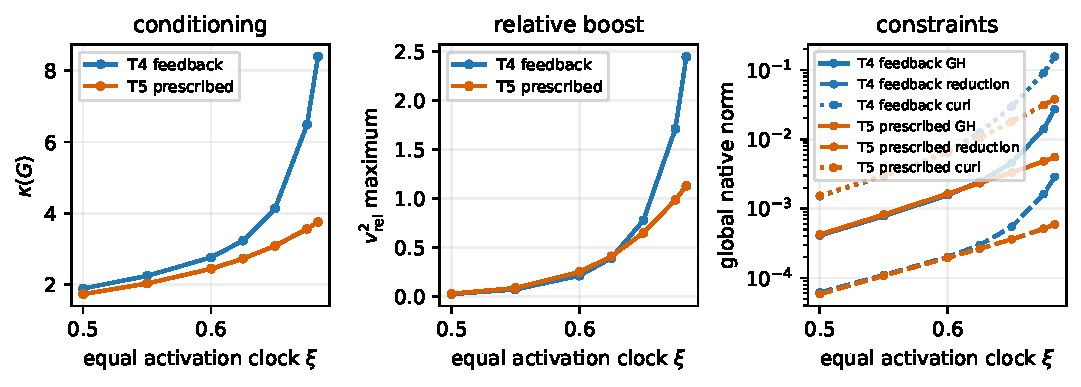
\includegraphics[width=0.98\textwidth]{fo_gh_artifacts/ref_gh_gaussian_reference_gamma2_20260824/figures/t4_t5_equal_activation.pdf}
\caption{Comparison at identical continuation clock $\xi$.  The controlled
path is not superior near the failure transition.}
\label{fig:equal}
\end{figure}

\subsection{Localization and causal exclusion}

The T4 accumulated characteristic distance is $3.48176M$, leaving
$20.51824M$ to the nearest outer face.  T5 accumulated $3.00307M$, leaving
$20.99693M$.  Thus neither outer boundary nor restart discontinuity can explain
these events.  Figure~\ref{fig:location} instead places the maxima of the GH,
reduction, curl, and reference-frame source diagnostics in the artificial
$0.30$--$0.60M$ stitching shell, well inside the finest-box face at $r=4M$.
This localization motivates the Gaussian hypothesis but does not prove it.

\begin{figure}[h]
\centering
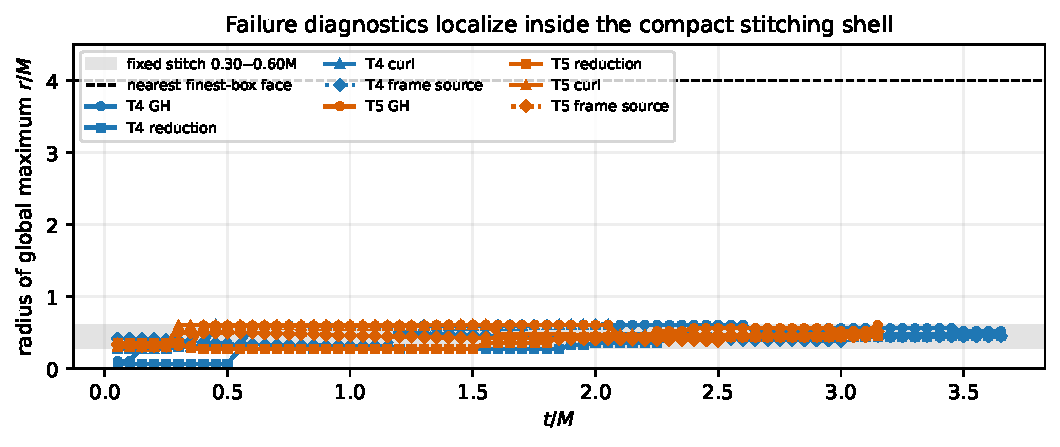
\includegraphics[width=0.96\textwidth]{fo_gh_artifacts/ref_gh_gaussian_reference_gamma2_20260824/figures/t4_t5_maximum_locations.pdf}
\caption{Radii of global diagnostic maxima.  Duplicate checkpoint rows are
deduplicated by time and diagnostic.  The refinement interface is not the
observed maximum location.}
\label{fig:location}
\end{figure}

\section{Current formulation and the missing standard
\texorpdfstring{$\gamma_2$}{gamma2} system}

Let $E_I=E_I{}^i\partial_i$ be the reference spatial frame, with dual
$\theta^I{}_i$ and commutator
$[E_I,E_J]=f_{IJ}{}^K E_K$.  The evolved variables are the frame metric
$\Psi_{AB}$, its normal-time variable $\Pi_{AB}$, and spatial derivative
$\Phi_{IAB}$.  The primary first-order constraints are
\begin{align}
  \CI &= E_I(\Psi_{AB})-\Phi_{IAB}, \\
  \CIJ &= E_I(\Phi_{JAB})-E_J(\Phi_{IAB})-f_{IJ}{}^K\Phi_{KAB}.
\end{align}
The second identity is the noncoordinate exterior derivative and is essential:
omitting $f_{IJ}{}^K$ creates a false curl signal.

The implemented system has effective $\gamma_1=-1$, gauge damping
$\gamma_0>0$, and $\gamma_2=0$.  Its compatible update differentiates the
discrete $\Psi$ right-hand side and adds
$(\partial_t E_I{}^p)\theta^J{}_p\Phi_J$.  The optional standard ordering
subtracts $\beta^J\CIJ$; this changes a curl-equivalent principal ordering but
does not supply standard reduction-constraint damping.  Component-wise KO
dissipation and component-wise SMR transfer also need not preserve
$\Phi=E(\Psi)$ in a varying frame.

\subsection{Coordinate standard system}

The complete first-order generalized-harmonic system of Lindblom, Scheel,
Kidder, Owen, and Rinne adds matched multiples of the reduction constraint to
all required equations.  Suppressing non-$\gamma_2$ sources, its principal
form is
\begin{align}
 \partial_t\psi_{ab}-(1+\gamma_1)\beta^k\partial_k\psi_{ab}
   &= -\alpha\Pi_{ab}-\gamma_1\beta^i\Phi_{iab}, \\
 \partial_t\Pi_{ab}-\beta^k\partial_k\Pi_{ab}
   +\alpha g^{ki}\partial_k\Phi_{iab}
   -\gamma_1\gamma_2\beta^k\partial_k\psi_{ab}
   &= \cdots-\gamma_1\gamma_2\beta^i\Phi_{iab}, \\
 \partial_t\Phi_{iab}-\beta^k\partial_k\Phi_{iab}
   +\alpha\partial_i\Pi_{ab}-\alpha\gamma_2\partial_i\psi_{ab}
   &= \cdots-\alpha\gamma_2\Phi_{iab}.
\end{align}
Symmetric hyperbolicity fixes $\gamma_3=\gamma_1\gamma_2$; this is why one
guessed local term is not an admissible comparator.

For $\gamma_1=-1$, the additional right-hand sides can be written directly in
constraint form:
\begin{align}
 \delta_{\gamma_2}(\partial_t\Psi_{AB}) &= 0, \\
 \delta_{\gamma_2}(\partial_t\Pi_{AB}) &=
       -\gamma_2\beta^I\CI, \\
 \delta_{\gamma_2}(\partial_t\Phi_{IAB}) &=
       +\alpha\gamma_2\CI. \label{eq:gamma2add}
\end{align}
Equation~\eqref{eq:gamma2add} is the compact implementation oracle, not a
license to omit the matching characteristic variables, diagnostics, and
boundary implications.

\subsection{Moving-frame and subsidiary requirements}

Because Eq.~\eqref{eq:gamma2add} is algebraic in the geometrically defined
constraint, it transforms cleanly to the reference frame.  All existing
time-dependent-frame and structure-coefficient terms remain part of the core
system.  If
\begin{equation}
 T_I{}^J=(\partial_t E_I{}^p)\theta^J{}_p,
\end{equation}
then the reduction subsidiary equation must include the corresponding
$T_I{}^J\mathcal C_J$ coupling, while the curl equation must include the
induced two-form action and the time derivative of the structure coefficients.
These are homogeneous constraint couplings; they cannot be dropped merely
because they vanish on the constraint surface.

The cited standard system gives the principal reduction-constraint speed
$(1+\gamma_1)\beta^n$.  Therefore, with $\gamma_1=-1$, its frozen-coefficient
subsidiary equation is locally
\begin{equation}
 \partial_t\CI \simeq -\alpha\gamma_2\CI,
 \label{eq:subsidiary}
\end{equation}
not literally $(\partial_t-\beta^I E_I)\CI$ unless a different convention or
constraint addition is deliberately chosen.  This is an important correction
to the schematic target in the controlling specification and must be resolved
by a symbolic principal-symbol oracle before production code is edited.

Taking the noncoordinate exterior derivative of
Eq.~\eqref{eq:subsidiary} gives, schematically,
\begin{equation}
 \partial_t\CIJ \simeq -\alpha\gamma_2\CIJ
  -2E_{[I}(\alpha\gamma_2)\mathcal C_{J]AB}
  +\hbox{homogeneous frame/shift couplings}.
\end{equation}
Thus the physically relevant curl is damped in the frozen-coefficient limit;
an independent direct curl penalty must not be invented without a separate
hyperbolicity proof.

The characteristic fields become
\begin{align}
 u^{\hat 0}_{AB}&=\Psi_{AB},\\
 u^{\hat 1\pm}_{AB}&=\Pi_{AB}\pm n^I\Phi_{IAB}-\gamma_2\Psi_{AB},\\
 u^{\hat 2}_{IAB}&=(\delta_I{}^J-n_In^J)\Phi_{JAB},
\end{align}
with speeds $-(1+\gamma_1)\beta^n$, $-\beta^n\pm\alpha$, and
$-\beta^n$, respectively.  The transformed symmetrizer contains
\begin{equation}
 \Lambda^2\,d\Psi^2+d\Pi^2-2\gamma_2\,d\Psi\,d\Pi
 +\bar g^{IJ}d\Phi_I d\Phi_J,
 \qquad \Lambda^2>\gamma_2^2.
\end{equation}
These formulas define unit tests for signs, characteristic reconstruction, and
positive definiteness.

\section{Gaussian-localized Schwarzschild reference}

The proposed reference replaces the sole narrow spatial transition by
\begin{equation}
 W(r;R_G)=\exp[-(r/R_G)^2],\qquad \rho=r/M,
\end{equation}
without compact support.  The time homotopy is $s(t)=S(t/\tau_{\rm ramp})$,
where, for $0<u<1$,
\begin{align}
 S(u)&=10u^3-15u^4+6u^5,\\
 S'(u)&=30u^2(1-u)^2,\\
 S''(u)&=60u(1-u)(1-2u).
\end{align}
The implementation must branch at the endpoints so that $\dot s=\ddot s=0$
exactly for $t\ge\tau_{\rm ramp}$ and before the ramp.

The unlocalized black-hole primitives are
\begin{align}
 \log\alpha_{\rm BH}&=(1-s)\log\alpha_W+s\log\alpha_T,\\
 \log\psi^2_{\rm BH}&=(1-s)\log\psi^2_W+s\log\psi^2_T,\\
 q^\beta_{\rm BH}&=s q^\beta_T,
\end{align}
and Gaussian localization relative to Minkowski is
\begin{align}
 \log\bar\alpha &= W\log\alpha_{\rm BH},\\
 \log\bar\psi^2 &= W\log\psi^2_{\rm BH},\\
 \bar q^\beta &= Wq^\beta_{\rm BH},\qquad
 \bar\beta^i=\bar q^\beta x^i.
\end{align}
It approaches the local hole reference at the puncture and Minkowski smoothly
for $r\gg R_G$.  The analytic radial jets are
\begin{align}
 W'&=-\frac{2r}{R_G^2}W,\\
 W''&=\left(\frac{4r^2}{R_G^4}-\frac{2}{R_G^2}\right)W,
\end{align}
while $\dot s=S'(u)/\tau_{\rm ramp}$ and
$\ddot s=S''(u)/\tau_{\rm ramp}^2$.  Products, logarithms, and exponentials
must use the existing analytic \code{ReferenceJet} algebra; finite differencing
the reference is outside scope.

Figure~\ref{fig:gaussian} illustrates the predeclared widths.  It is a design
plot only.  The broad derivative scales are controlled by $R_G^{-1}$ and
$R_G^{-2}$, which the reference-only scan must distinguish from logarithmic or
algebraic grid-scale growth.

\begin{figure}[h]
\centering
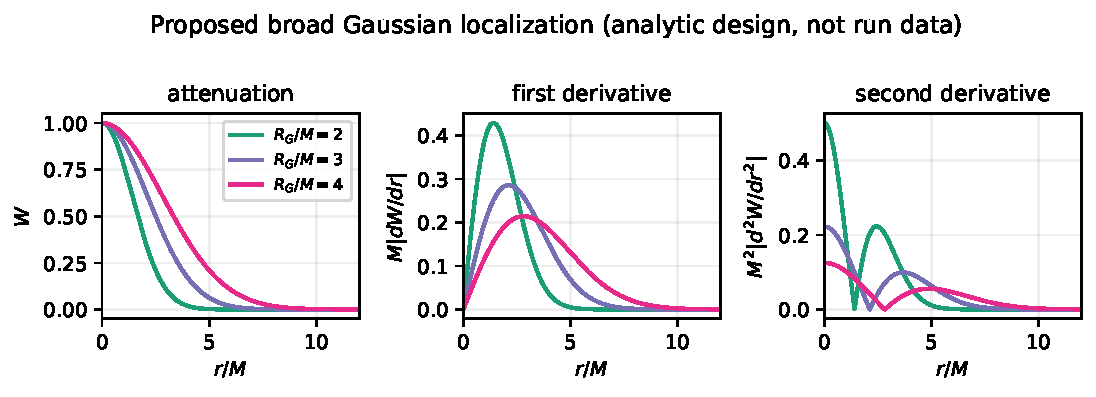
\includegraphics[width=0.98\textwidth]{fo_gh_artifacts/ref_gh_gaussian_reference_gamma2_20260824/figures/gaussian_reference_profiles.pdf}
\caption{Analytic Gaussian attenuation and derivative magnitudes for the
fixed proposed widths.  No evolution data enter this figure.}
\label{fig:gaussian}
\end{figure}

\section{GH-compatible initialization with a mismatched reference}

The physical initial data remain exact isotropic Schwarzschild wormhole data:
\begin{equation}
 \gamma_{ij}=\psi_W^4\delta_{ij},\quad
 \alpha=\psi_W^{-2},\quad \beta^i=0,\quad K_{ij}=0.
\end{equation}
Because the Gaussian reference becomes Minkowski outside its local region,
$\Psi=\eta$, $\Pi=0$, and $\Phi=0$ are generally false.  A reusable
ADM-plus-reference initializer should proceed as follows.

\begin{enumerate}
\item Construct the physical coordinate four-metric,
\begin{align}
 g_{00}&=-\alpha^2+\gamma_{ij}\beta^i\beta^j,&
 g_{0i}&=\gamma_{ij}\beta^j,&g_{ij}&=\gamma_{ij}.
\end{align}
\item Transform with the analytic reference frame:
$\Psi_{AB}=e_A{}^a e_B{}^b g_{ab}$.
\item Differentiate the analytic physical metric and reference frame, then
set $\Phi_{IAB}=E_I{}^i\partial_i\Psi_{AB}$.  This step includes derivatives
of both $g_{ab}$ and $e_A{}^a$.
\item Use
$\partial_t\gamma_{ij}=-2\alpha K_{ij}+\mathcal L_\beta\gamma_{ij}$ to fix
the six spatial-metric time derivatives.  Determine the remaining four
$\partial_tg_{0\mu}$ by solving the four background-covariant GH gauge
constraints $\CGH=0$.  Equivalently, solve the resulting ten-by-ten linear
map for $\Pi_{AB}$ after including the analytic $\partial_t e_A{}^a$ terms.
Do not guess $\Pi$.
\item Reconstruct ADM variables and require the intended
$(\alpha,\beta^i,\gamma_{ij},K_{ij})$, roundoff-level analytic $\Phi$
definition residual, roundoff/truncation-oracle GH constraint, and existing
Schwarzschild ADM-constraint accuracy.
\end{enumerate}

This linear solve is the correct place to expose rank, conditioning, and sign
failures.  It is also the reusable architecture needed by a future composite
binary reference; a generic Cholesky tetrad is deliberately not part of the
present task.

\section{Predeclared gates and fixed experiments}
\label{sec:gates}

The Gaussian and $\gamma_2$ hypotheses must be separated before being
combined.  Table~\ref{tab:status} records the current evidence boundary.

\begin{table}[h]
\centering
\caption{Completion state at report generation.}
\label{tab:status}
\begin{tabular}{p{0.55\textwidth}p{0.18\textwidth}p{0.18\textwidth}}
\toprule
gate & state & evidence \\
\midrule
existing source/moving-reference/PVC/restart gates & \passed & committed logs \\
T4 medium feedback continuation & \failed & job 8777607 \\
T5 medium prescribed continuation & \failed & job 8777824 \\
Gaussian reference and analytic jet oracle & \notrun & no implementation \\
GH-compatible mismatched-reference initializer & \notrun & no implementation \\
standard moving-frame $\gamma_2$ manufactured tests & \notrun & no implementation \\
Gaussian $3\times3$ reference-only scan & \notrun & no results \\
Gaussian $3\times3$ medium evolution matrix & \notrun & no results \\
Gaussian/$\gamma_2$ black-hole ablation and causal $2\times2$ & \notrun & no results \\
conditional three-resolution gate & disallowed now & prerequisite unmet \\
\bottomrule
\end{tabular}
\end{table}

\subsection{Reference-only matrix}

Before evolution, scan exactly $R_G/M\in\{2,3,4\}$ and
$\tau_{\rm ramp}/M\in\{4,8,16\}$ at
$s\in\{0,0.25,0.5,0.75,1\}$ and cell-centered radii for
$h/M\in\{1/16,1/24,1/32,1/48\}$.  Record values and locations of $|W'|$,
$|W''|$, spin connection and derivative, reference Ricci/Riemann, every source
sector, and the total source.  Compare the maxima with the old compact stitch
and fit the innermost resolution dependence without expanding the matrix after
seeing results.

\subsection{Manufactured off-constraint tests}

Plant reduction and curl violations separately in flat, spatially varying,
and genuinely time-dependent frames for $\gamma_2M=0,0.5,1.0$.  The
frozen-coefficient reduction norm must follow the decay rate derived from
Eq.~\eqref{eq:subsidiary}; curl behavior must follow the exterior-derivative
subsidiary system.  Repeat selected cases with KO off/on and record an RHS
split into core, moving-frame, $\gamma_2$, and KO contributions.  A
zero-constraint exact solution is not a sufficient test.

\subsection{Black-hole matrices}

First run the fixed Gaussian $3\times3$ medium matrix with standard ordering,
$\gamma_2=0$, controller off, and $\delta_q=\delta_p=0$.  Rank cases
lexicographically by: successful full activation plus hold, then maximum
relative boost, condition number, GH/curl growth, and reference/source maxima.
Promote at most two candidates.  Only those candidates receive
$\gamma_2M=0,0.5,1.0$; $2.0$ is allowed once only under the predeclared narrow
condition.  Finally compare old/Gaussian crossed with $\gamma_2M=0/1$ at equal
time and activation.

The three-resolution $M/16$, $M/24$, $M/32$ gate is conditional on one medium
candidate reaching full activation plus a $2M$ hold with controlled native
constraints.  Until then there is no convergence campaign to report.

\section{Portability, SMR, and boundary implications}

Aurora qualification must show Level Zero SYCL execution on each requested PVC
tile, not merely configuration or compilation.  Runtime evidence must retain
source and Kokkos SHAs, compiler/runtime/device versions, selectors, rank-to-tile
mapping, binary hashes, checkpoints, and resource observations.  The current
T4/T5 evidence satisfies this for those exact runs only.

Two discrete constraint-injection channels require instrumentation:
component-wise KO does not commute with $\Phi=E(\Psi)$ in a spatially varying
frame, and AthenaK transfers all 50 evolved components independently across
SMR.  Neither mechanism is established as the cause of T4/T5 because maxima
lie near $r=0.5M$, far inside the nearest interface.  If a manufactured or
Gaussian run localizes first growth at an interface, the black-hole gate must
stop for a separate constraint-compatible transfer/gradient-repair task.

The existing outer treatment is not a constraint-preserving GH boundary.
Although causally irrelevant to T4/T5, it remains a future long-time
qualification blocker.  Every subsequent run must integrate maximum
characteristic speed and state the remaining coordinate distance rather than
calling the boundary remote by inspection.

\section{Reproduction and artifact map}

From the repository root, regenerate all figures and compile the report with:
\begin{verbatim}
python3 scripts/ref_gh/plot_ref_gh_gaussian_gamma2_report.py
cd docs
pdflatex -interaction=nonstopmode -halt-on-error \
  ref_gh_gaussian_reference_gamma2_20260824.tex
pdflatex -interaction=nonstopmode -halt-on-error \
  ref_gh_gaussian_reference_gamma2_20260824.tex
\end{verbatim}
The script reads only committed T4/T5 histories and the committed equal-clock
comparison JSON.  The generated plot PDFs/PNGs and this report PDF live under
\path{docs/fo_gh_artifacts/ref_gh_gaussian_reference_gamma2_20260824/}
or alongside this source, as recorded in the artifact manifest.

The large Aurora outputs remain intentionally outside Git:
\begingroup\footnotesize\sloppy
\begin{itemize}
\item T4: \path{/lus/flare/projects/CompactBinaryMerger/hzhu/refgh_feedback_continuation_20260823_2466879e_v1/runs/t4_feedback_outer24_8777607.aurora-pbs-0001.hostmgmt.cm.aurora.alcf.anl.gov}
\item T5: \path{/lus/flare/projects/CompactBinaryMerger/hzhu/refgh_feedback_continuation_20260823_2466879e_v1/runs/t5_prescribed_outer24_8777824.aurora-pbs-0001.hostmgmt.cm.aurora.alcf.anl.gov}
\end{itemize}
\endgroup

\section{Conclusion}

The compact fixed-core evidence rejects both tested continuation paths but
does not identify a unique cause.  The strongest observations are the
stitch-shell localization and the absence of standard $\gamma_2$ damping;
the strongest structural risks are moving-frame off-constraint propagation,
component-wise KO, and independent SMR transfer.  The Gaussian and
$\gamma_2$ hypotheses must therefore be tested independently with analytic
jets, a GH-compatible initializer, planted off-constraint oracles, and fixed
predeclared matrices.  At this point the correct scientific statement is:
\begin{center}
\fbox{\parbox{0.88\textwidth}{No Gaussian-reference result, no
$\gamma_2$ damping result, no convergent trumpet evolution, and no long-time
stability result has been established.}}
\end{center}

\begin{thebibliography}{9}
\bibitem{Lindblom2006}
L.~Lindblom, M.~A.~Scheel, L.~E.~Kidder, R.~Owen, and O.~Rinne,
``A New Generalized Harmonic Evolution System,''
Class. Quantum Grav. 23 (2006),
\url{https://arxiv.org/abs/gr-qc/0512093}.
\end{thebibliography}

\end{document}
